\documentclass{article}%
\usepackage[T1]{fontenc}%
\usepackage[utf8]{inputenc}%
\usepackage{lmodern}%
\usepackage{textcomp}%
\usepackage{lastpage}%
\usepackage[head=40pt,margin=0.5in,bottom=0.6in]{geometry}%
\usepackage{graphicx}%
%
\title{\textbf{La ONU aprobó ayuda de emergencia humanitaria para Venezuela}}%
\author{El Nacional Web}%
\date{26/11/2018}%
%
\begin{document}%
\normalsize%
\maketitle%
\textbf{URL: }%
http://www.el{-}nacional.com/noticias/mundo/onu{-}aprobo{-}ayuda{-}emergencia{-}humanitaria{-}para{-}venezuela\_261168\newline%
%
\textbf{Periodico: }%
EN, %
ID: %
261168, %
Seccion: %
Mundo\newline%
%
\textbf{Palabras Claves: }%
Crisis humanitaria, ONU\newline%
%
\textbf{Derecho: }%
18, %
Otros Derechos: %
CONTEXTO, %
Sub Derechos: %
\newline%
%
\textbf{EP: }%
NO\newline%
\newline%
%
\textbf{\textit{Los fondos proceden del Fondo Común de Respuesta a Emergencias de la Organización de las Naciones Unidas y financiarán programas de ayuda a venezolanos}}%
\newline%
\newline%
%
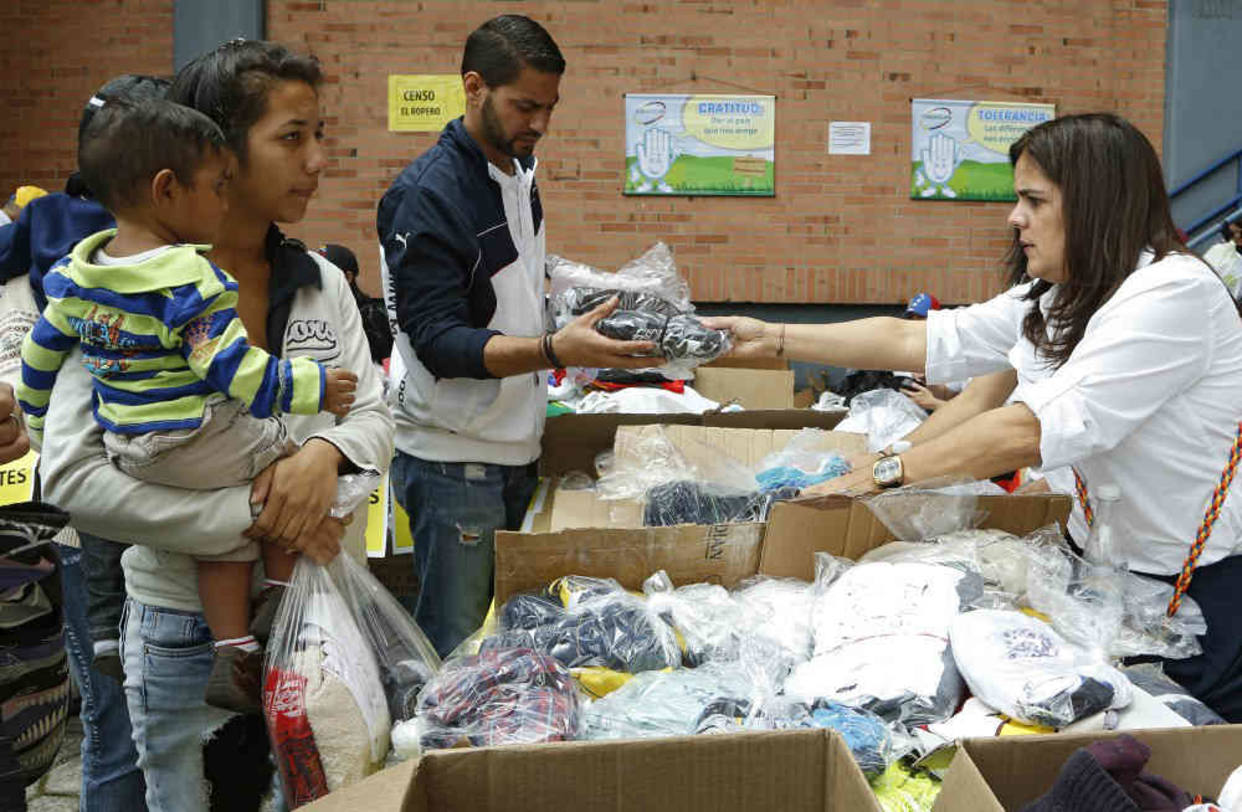
\includegraphics[width=300px]{222.jpg}%
\newline%
%
La Organización de las Naciones Unidas (ONU) anunció este lunes la aprobación del primer financiamiento de ayuda humanitaria para Venezuela a través de programas humanitarios, informó~Reuters.%
\newline%
%
Una portavoz de la organización indicó que el presupuesto aprobado fue de 9,2 millones de dólares, y será destinado para organizaciones que atiendan la asistencia en salud y nutrición a menos de edad y mujeres, destacó la agencia de noticias.%
\newline%
%
Los fondos, que fueron tomados del Fondo Común de Respuesta a Emergencias, se ofrecen para apoyar a organizaciones no gubernamentales que tengan el objetivo de ayudar a personas en condiciones de vulnerabilidad como niños, mujeres embarazadas y personas que se desplazan en comunidades fronterizas, señaló la agencia.%
\newline%
%
Es la primera vez que la ONU aprueba una ayuda de esta magnitud para el país y numerosas solicitudes. El gobierno de Nicolás Maduro ha rechazado la ayuda de otras naciones debido a la negación de la existencia de la crisis humanitaria del país.%
\newline%
%
Con información de~Reuters%
\newline%
%
\end{document}